\chapter[Considerações Finais]{CONSIDERAÇÕES FINAIS}

Minha trajetória ao longo da \ac{ages} foi a experiência mais significativa da minha graduação em Engenharia de Software. Diferentemente de outros cursos da área da computação, a Engenharia de Software oferece, por meio da Agência, a oportunidade de exercitar na prática os conhecimentos adquiridos em sala de aula, em um ambiente muito próximo ao do mercado de trabalho, com clientes e entregas reais. Ao percorrer os quatro papéis da Agência, dos primeiros passos como \ac{ages} I ao encerramento do ciclo como \ac{ages} IV, amadureci competências técnicas e interpessoais que hoje considero fundamentais para a minha formação.

No aspecto técnico, cada passagem me colocou diante de um desafio distinto. No Focus, dei meus primeiros passos no desenvolvimento, aprendendo uma \textit{stack} do zero e ainda muito dependente do apoio de colegas mais experientes. No Decola, atuei mais próximo dos dados e do \textit{frontend}, já com autonomia para assumir tarefas sozinho. No Totem Interativo, assumi a frente de arquitetura, tomando decisões estruturais e orientando os \ac{ages} menores. Por fim, no Estudify, deixei o código em segundo plano para me dedicar à gestão da equipe e à coordenação das entregas.

No campo interpessoal, a evolução foi igualmente marcante. Comecei a graduação como uma pessoa reservada e de perfil predominantemente técnico. Ao longo das passagens pela \ac{ages}, desenvolvi minha comunicação e meu trabalho em equipe, e foi nos papéis de \ac{ages} III e IV que precisei exercer liderança de verdade. Aprender a delegar, em vez de centralizar tudo em mim, foi o aprendizado que levei mais tempo para incorporar, e um dos mais valiosos.

Um aprendizado que atravessou toda a minha trajetória diz respeito à forma como a viabilidade técnica do escopo é tratada nas fases iniciais da \ac{ages}. O documento de abertura, que estabelece o que será construído, é elaborado pela equipe da Agência em conjunto com o cliente, antes que os alunos responsáveis pela execução sejam envolvidos. É verdade que, após receber esse documento, o time tem espaço para negociar com o cliente o que será ou não desenvolvido, ajustando o escopo conforme a capacidade e as prioridades. Esse mecanismo funciona bem para questões de tamanho e prioridade, mas não resolve o problema mais crítico: quando um requisito é tecnicamente inviável. Vivenciei isso em mais de uma passagem. No Focus, a proposta previa que o aplicativo monitorasse o uso do celular de forma ininterrupta, recurso que os próprios sistemas operacionais móveis restringem por questões de privacidade e arquitetura. No Totem Interativo, o \textit{stakeholder} desejava que o mapa fosse gerado a partir da planta baixa do evento em formato DWG, do AutoCAD, o que dependeria de uma \ac{api} paga e proprietária para seguir funcionando. Nesses casos, não se tratava de negociar prazo ou prioridade, mas de uma impossibilidade técnica que só foi percebida durante a execução, com a \textit{sprint} já em andamento, obrigando o time a recuar e repensar a solução.

Disso decorre minha principal sugestão de melhoria ao processo da \ac{ages}: reforçar a validação técnica de viabilidade antes de o documento de abertura ser fechado com o cliente. A renegociação de escopo já existente é valiosa, mas pressupõe que o que está no papel é construível, e nem sempre é. Uma verificação prévia das restrições de plataforma, de licenciamento e de prazo evitaria que premissas inviáveis chegassem ao time como compromissos já assumidos com o cliente, poupando o retrabalho de descobrir o problema tarde demais. Em contrapartida, deixo registrado meu reconhecimento: a \ac{ages} é o maior diferencial do curso e o espaço mais próximo da realidade profissional que tive durante a graduação.

A percepção dessa evolução pode ser observada na Figura~\ref{fig:radar-ages}, que sintetiza minha avaliação sobre as principais competências técnicas e interpessoais em cada passagem pela Agência. Nota-se um crescimento consistente das habilidades técnicas, com destaque para a \ac{ages} III, em que assumi a responsabilidade pela arquitetura do projeto. Já na \ac{ages} IV, evidencia-se o fortalecimento das competências de comunicação, liderança e gestão de equipe, refletindo o papel mais estratégico que exerci no Estudify.

\begin{figure}[H]
    \centering
    \small
    \caption{Gráfico radar da evolução do aluno na AGES}
    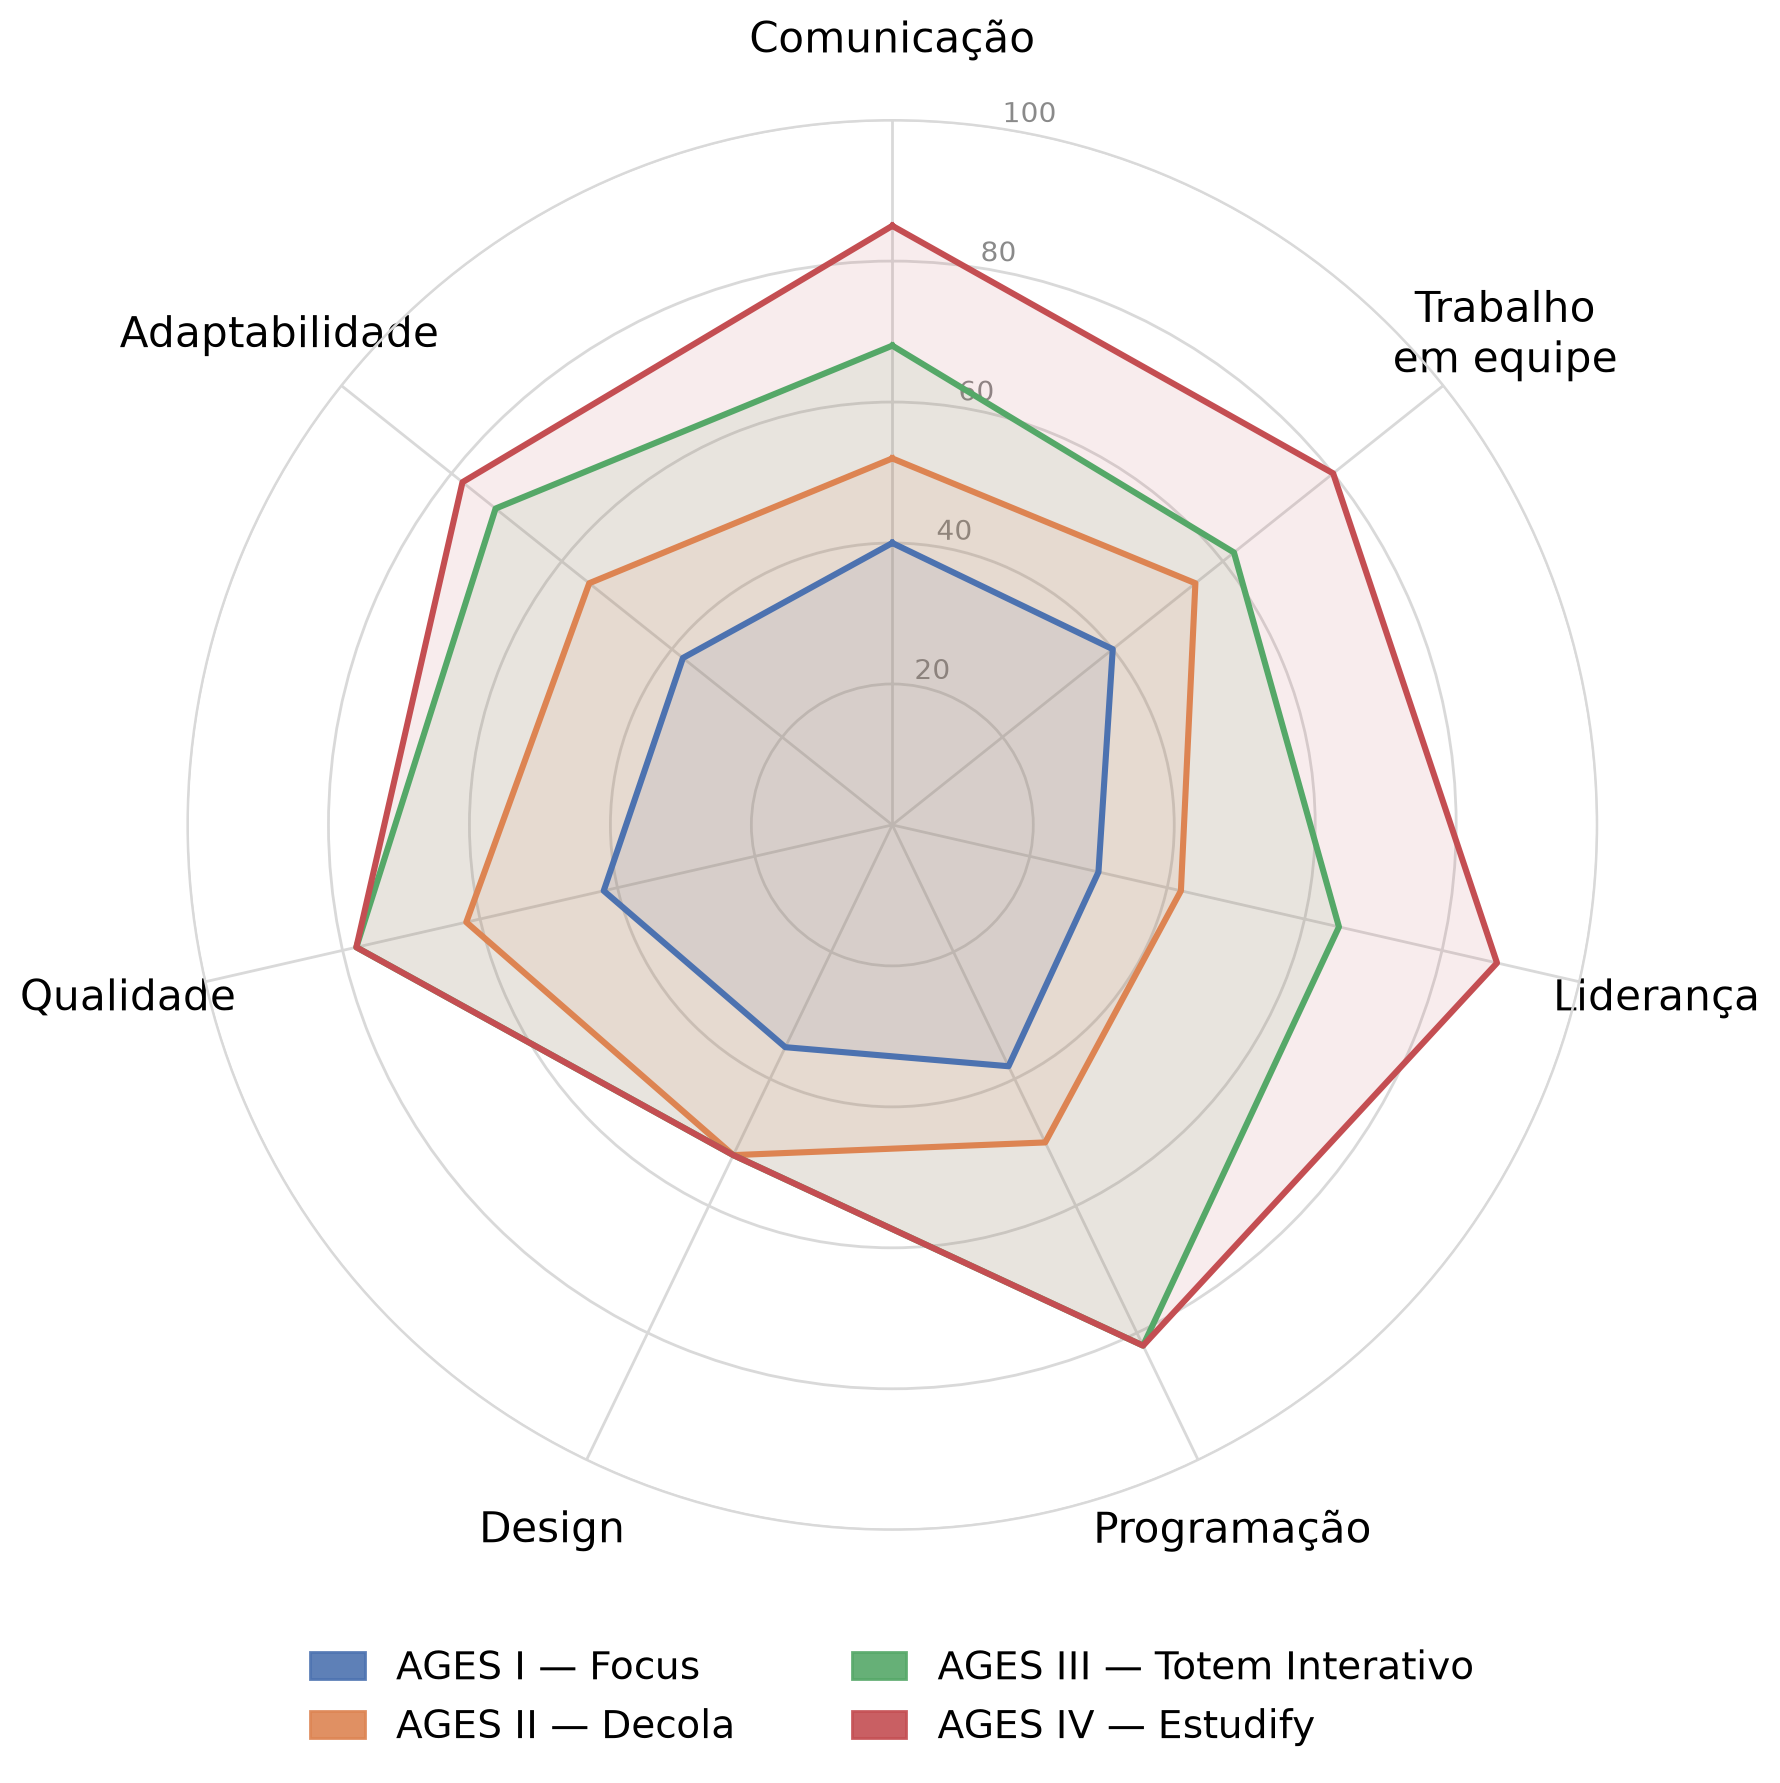
\includegraphics[width=0.85\linewidth]{conteudo/6 - consideracoes/images/fig-radar-ages.png}

    Fonte: Autor
    \label{fig:radar-ages}
\end{figure}

Concluo esta jornada com gratidão e um forte senso de propósito. A \ac{ages} não apenas me preparou para o mercado de trabalho, mas moldou minha visão sobre como desejo atuar nele, mostrando-me que a evolução profissional, assim como a liderança, é um processo contínuo de aprendizado. Encerro o ciclo com a certeza de ter me tornado um profissional mais completo e preparado para os desafios que virão.
